\documentclass{overturerepsec}
\usepackage{url}
\usepackage{graphics}
\usepackage{times}
\usepackage{listings}
\usepackage{color}
\usepackage{graphicx}
\usepackage{latexsym}
\usepackage{longtable} % ,multirow}

\newcommand{\vdmtools}{VDMTools}
\newcommand{\vdmstyle}[1]{\texttt{#1}}
\newcounter{exerciseno}

%\newcommand{\Exercise}[1]{%
%    \textbf{Exercise \thechapter.\theexerciseno}
%   \refstepcounter{exerciseno} #1 $\Box$\\ }%}
%\newcommand{\initexercise}{\setcounter{exerciseno}{0}}
%\newcounter{exerciseno}

\newcommand\thebookexercise{\thechapter.\arabic{exerciseno}}
\newenvironment{myexercise}{\par
  \refstepcounter{exerciseno}%
  \indent\textbf{Exercise\ \thebookexercise}\enskip}{$\Box$\\
}
\newenvironment{myhardexercise}{\par
  \refstepcounter{exerciseno}%
  \indent\textbf{Exercise\ \thebookexercise $\star$}\enskip}{$\Box$\\
}
\newcommand{\initexercise}{\setcounter{exerciseno}{0}}
\newenvironment{mysolution}{
} %% This will be replaced by a perl script extracting the solutions
  %% and inserting them automatically into the solutions chapter.
 
%\newcommand{\insertcommentedvdm*}[2]{}
  %% This macro is identified by perl script which will move the
  %% parameter to the solutions chapter.
% definition of VDM++, JavaCC, JJTree, JTB, ANTLR and SableCC for listings
\lstdefinelanguage{VDM++}
  {morekeywords={act, active, fin, req, waiting, abs, all, allsuper, always, and, answer, 
     assumption, async, atomic, be, bool, by, card, cases, char, class, comp, compose, conc, cycles,
     dcl, def, definitions, del, dinter, div, dlmodule, do, dom, dunion, duration, effect, elems, else, elseif, end,
     error, errs, exists, exists1, exit, exports, ext, floor, for, forall, from, functions, 
     general, hd, if, imports, in, inds, infer, init, inmap, input, instance, int, inter, inv, inverse, iota, is, 
     isofbaseclass, isofclass, inv, inverse, lambda, len, let, map, measure, mu,
     mutex, mod, module, nat, nat1, new, merge, 
     munion, not, of, operations, or, others, per, periodic, post, power, pre, pref, 
     private, protected, public, qsync, rd, responsibility, return, reverse,  
     sameclass, parameters, psubset, rem, renamed, rng, sel, self, seq, seq1, set, skip, specified, st, 
     start, startlist, state, static, subclass, subset, subtrace, sync, system, then, thread, 
     threadid, time, tixe, tl, to, token, traces, trap, types, undefined,
     union, uselib, using, values, 
     variables, while, with, wr, yet, RESULT, false, true, nil, periodic pref, rat, real},
   %keywordsprefix=mk\_,
   %keywordsprefix=a\_,
   %keywordsprefix=t\_,
   %keywordsprefix=w\_,
   sensitive,
   morecomment=[l]--,
   morestring=[b]",
   morestring=[b]',
  }[keywords,comments,strings]
\lstdefinelanguage{JavaCC}
  {morekeywords={options, PARSER\_BEGIN, PARSER\_END, SKIP, TOKEN},
   sensitive=false,
  }[keywords]

% define the layout for listings
\lstdefinestyle{tool}{basicstyle=\ttfamily,
                         frame=trBL, 
			 showstringspaces=false, 
			 frameround=ffff, 
			 framexleftmargin=0mm, 
			 framexrightmargin=0mm}
\lstdefinestyle{mystyle}{basicstyle=\ttfamily,
                         frame=trBL, 
%                         numbers=left, 
%			 gobble=0, 
			 showstringspaces=false, 
%			 linewidth=\textwidth, 
			 frameround=fttt, 
			 aboveskip=5mm,
			 belowskip=5mm,
			 framexleftmargin=0mm, 
			 framexrightmargin=0mm}
%\lstdefinestyle{mystyle}{basicstyle=\sffamily\small,
%			 frame=tb,
%                         numbers=left,
%			 gobble=0,
%			 showstringspaces=false,
%			 linewidth=345pt,
%			 frameround=ffff,
%			 framexleftmargin=8mm,
%			 framexrightmargin=8mm,
%			 framextopmargin=1mm,
%			 framexbottommargin=1mm,
%			 aboveskip=7mm,
%			 belowskip=5mm,
%			 xleftmargin=10mm,}

\lstset{style=mystyle}
\lstset{language=VDM++}
\lstset{alsolanguage=Java}
% The command below enables you to escape into normal LaTeX mode inside your 



%%%%%%%%%%%%%%%%%% Commands for bibtex %%%%%%%%%%%%%%%%%%%%%%%
%************************************************************************
%                                                                       *
%       Bibliography and Terminology supporting commands                *
%                                                                       *
%************************************************************************

\newcommand{\bthisbibliography}[1]{\chapter*{References}%
   \begin {list} {}%
     {\settowidth {\labelwidth} {[#1]XX}%
      \setlength {\leftmargin} {\labelwidth}%
      \addtolength{\leftmargin} {\labelsep}%
      \setlength {\parsep} {1ex}%
      \setlength {\itemsep} {2ex}%
     }
  }
\newcommand{\ethisbibliography}{\end{list}}
\newcommand{\refitem}[2]
  {\bibitem[#1]{#2}}

%\newcommand{\Exercise}[1]{%
%    \textbf{Exercise \thechapter.\theexerciseno}
%   \refstepcounter{exerciseno} #1 $\Box$\\ }%}
%\newcommand{\initexercise}{\setcounter{exerciseno}{0}}

\newcommand{\experience}[1]{%
\begin{center}
\fbox{
\begin{minipage}[t]{.8\textwidth}
#1
\end{minipage}}
\end{center}}

\usepackage{fancyhdr}

\pagestyle{fancy}
\fancyhead{}
\fancyhead[LO]{\leftmark}
\fancyhead[RE]{Tutorial to Overture/VDM-RT}
\fancyhead[RO,LE]{\resizebox{0.05\textwidth}{!}{
\includegraphics{overture}}}
\fancyfoot[C]{\thepage}

\begin{document}
 
\title{Tutorial for Overture/VDM-RT}
\author{Peter Gorm Larsen\\
        %\and
        John Fitzgerald \\
        %\and
        Sune Wolff\\
        %\and
        Nick Battle\\
        Kenneth Lausdahl\\
        Augusto Ribeiro\\
        Kenneth Pierce}

\date{April 2013}

%\frontmatter
\reportno{TR-005}     

\pagenumbering{roman}
\maketitle
%\addtocounter{page}{2}

{\textbf{Document history}}

\begin{tabular}{|l|l|l|l|}\hline
Month   & Year & Version & Version of Overture.exe \\ \hline
January & 2010 &   & 0.1.5 \\ \hline
March   & 2010     & & 0.2   \\ \hline
May     & 2010 & 1 & 0.2  \\ \hline
February& 2011 & 2 & 1.0.0\\ \hline
April   & 2013 &3  & 2.0.0\\ \hline
\end{tabular}

\tableofcontents
\newpage
% \include{foreword/foreword}

%\cleardoublepage
%\mainmatter
%\lhead{\nouppercase{\rightmark}}
%\rhead{\nouppercase{\leftmark}}


%\pagestyle{fancy}
%\fancyhead{}
%\fancyhead[LO]{\leftmark}
%\fancyhead[RE]{Validated Designs for Object-oriented Systems}
%\fancyhead[RO,LE]{\thepage}
%\fancyfoot{}
%%\fancyfoot[LE,RO]{\thepage}

\pagenumbering{arabic} 
\setcounter{page}{1}
\addtocounter{chapter}{2}

% $Revision: 1.28 $
\chapter{Overture Tool Support for VDM-RT: an Introductory Guide}\label{cha:toolbox}
% vppinput[guide/test1.vpp]
\initexercise

\section*{Preamble}

This is an introduction to the Overture Integrated Development
Environment (IDE) and its facilities for supporting modelling and
analysis in VDM-RT the VDM extended language for modelling real-time
systems, formerly known as VICE~(VDM in Constrained Environments). It
may be used as a substitute for Chapter 3 of ``Validated Designs for
Object-oriented Systems''\footnote{John Fitzgerald, Peter Gorm Larsen,
  Paul Mukherjee, Nico Plat and Marcel Verhoef. \emph{Validated
    Designs for Object-oriented Systems}, Springer, New York. 2005,
  ISBN 1-85233-881-4.} or as a free-standing guide. Additional material
is available on the book's web
site\footnote{\url{www.vdmbook.com}.}. Throughout this guide we will refer to
the textbook as ``the book'' and the book's web site simply as ``the
web site''.

We use examples based on an \emph{in-car navigation} case study and
VDM-RT model presented in Appendix~\ref{app:navigation}. 

We introduce the features of Overture that support the combination of
formal modelling in VDM++ with object-oriented design using UML. This
is done by providing a ``hands-on'' tour of Overture, providing enough
detail to allow you to use Overture for serious applications,
including the exercises in the book. However, this is by no means a
complete guide to Overture\footnote{Note that the Overture tool suite support three
  different VDM dialects; VDM-SL (Specification Language), VDM++ and
  VDM-RT (Real Time) so although this tutorial illustrate how to use
  Overture with VDM-RT models you will see multiple references to
  these dialects throughout this tutorial.}; more information can be obtained
from~\url{www.overturetool.org}.



\section{Introduction}

In this chapter, an in-car radio navigation system which supports the Traffic Message Channel (TMC) will used as example. 

The system is composed of three main clusters of functionality; 
\begin{itemize}
\item The man-machine interface (MMI) takes care of user interaction such as handling key press input and graphical display output. 
\item The navigation is responsible for destination entry, route planning and turn-by-turn guidance. 
\item The radio is responsible for basic tuner and volume control as well as handling traffic information from the TMC.
\end{itemize}

Figure~\ref{fig:navigationoverview} gives an overview of the in-car navigation system. 

\begin{figure}[!h]
\begin{center}
  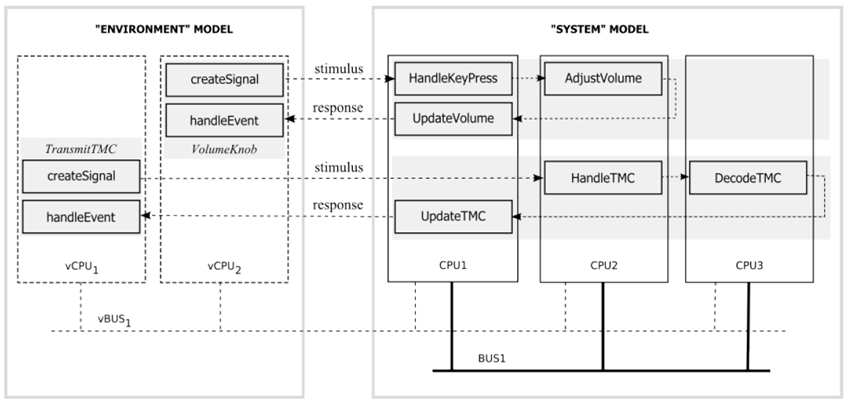
\includegraphics[width=4.5in]{figures/CarNavigationOverview}
  \caption[labelInTOC]{Car Navigation System Overview}
  \label{fig:navigationoverview}
\end{center}
\end{figure}

The system must be able to support the following three use cases:

\begin{description}
\item[\textbf{Change Volume:}] The user turns the rotary button and expects near instant audible feedback from the system. Furthermore, the visual feedback
(the volume setting on the screen) should be timely and synchronized with the
audible feedback.
\item[\textbf{Address Look-up:}] Destination entry is supported by a smart ``typewriter'' style interface. By turning a knob the user can move from letter to letter; by pressing it the user will select the currently highlighted letter. The map database is searched for each letter that is selected and only those letters in the on-screen alphabet are enabled that are potential next letters in the list.
\item[\textbf{TMC Message Handling:}] Digital traffic information is important for in-car radio navigation systems. It enables features such as automatic re-planning of the planned route in case a traffic jam occurs ahead. It is also increasingly important to enhance road safety by warning the driver, for example when a ghost driver is spotted just ahead on the planned route. TMC is such a digital traffic information service.
\end{description}

When developing a Real-time model, it is adviced to create an object-oriented model first outside the real-time domain. This will enable the developer to focus on the structure of the system as well as eliminating any concurrency issued before moving on to the real-time domain. This proposed process is described in much more detail in \cite{Larsen&09b}.

The rest of this chapter has the following outline; Section~\ref{sec:install} describes how to obtain the Overture tools.
Section~\ref{sec:vdmsupport} provides an initial introduction to the
terminology used by Eclipse tools like Overture. 
%% This section may be
%% skipped by readers who are already familiar with using Eclipse
%% tools. 
Section~\ref{sec:fromUMLtoVDM} shows how VDM-RT models can be
connected to UML.
Section~\ref{sec:debugging} describes the process of testing and
debugging VDM-RT models using Overture. Section~\ref{sec:RTLV} goes on
to show the Real-Time Log Viewer which gives a graphical presentation
of thread execution.
%Section~\ref{sec:CT} shows how parts of the test process can be
%automated using Overture's combinatorial testing feature.
Section~\ref{sec:PO} demonstrates the automatic generation of the
additional checks (called \emph{proof obligations}) needed to ensure
that a model is consistent.  Finally, Section~\ref{sec:cmdline}
illustrates how parts of Overture's functionality can be accessed from
a command line, including support for test coverage analysis which is
not currently available from the Overture IDE.

\section{Obtaining the Overture Tools}\label{sec:install}

In order to run the examples and exercises presented in the book, you
will need to download the Overture tools from the Internet.
%In order to run the software on your own computer you need to follow
%these instructions:
Overture is an open source tool, developed by volunteers and built on
the Eclipse platform. The project is managed on
SourceForge\footnote{\url{https://sourceforge.net/projects/overture/}}.
The best way to run Overture is to download a special version of
Eclipse with the Overture functionality already pre-installed. If you
go to:
  \begin{quote}
  \texttt{http://sourceforge.net/projects/overture/files/}
  \end{quote}
  \noindent you will find pre-installed versions of Overture for
  Windows, Linux and Mac\footnote{It is planned to develop an update
    facility, allowing updates to be applied directly from within the
    Overture tools without requiring a reinstallation. However, this
    can be a risky process because of the dependencies on non-Overture
    components and so is not yet supported.}.

A library of sample VDM-RT models, including all those needed
for the exercises in the book, is available and can be downloaded from
SourceForge under the \texttt{examplesRT.zip} file using the
URL\footnote{The library files are created to be used with Eclipse,
  but can be opened with file compression programs like \texttt{Winrar} on
  Windows.}:
\begin{quote}
\url{https://sf.net/projects/overture/files/Examples/}
\end{quote}
You can import the example library zip folder as described in
Section~\ref{sec:vdmsupport}.  Finally, the web site
\texttt{www.vdmbook.com} contains all the examples used in this book
as plain text files but these are also all present in the above
mentioned zip file. Finally, in order to make use of the
test coverage feature described in Section~\ref{sec:testcov} it is
necessary to have the text processing system called \LaTeX\ and its
\texttt{pdflatex} feature. This can for example be obtained from:
\begin{quote}
\url{http://miktex.org/2.8/}
\end{quote}

\paragraph{Note for \vdmtools$^{\mbox{\small\textbf{{\textregistered}}}}$ users.} 
Overture provides a new open source VDM tool set, but it can also work
in conjunction with the
\vdmtools$^{\mbox{\small\textbf{{\textregistered}}}}$
tool set originally developed by IFAD A/S and now maintained and
developed by CSK Systems~(see
\texttt{http://www.vdmtools.jp/en/}). Overture accesses VDMTools
functionality via a remote API, and the integration is to some extent
limited by the API capabilities. However, the additional features
provided by the Overture GUI make it worth considering as a front end
to the VDMTools functionality.
 
\section{Using the Overture Perspective}\label{sec:vdmsupport}

Eclipse is an open source platform based on a \emph{workbench} that
provides a common look and feel for a large collection of extension
products. Thus if a user is familiar with one Eclipse-based product,
it will generally be easy to start using a different product on the
same workbench. The Eclipse workbench consists of several panels
called \emph{views}, such as the Script Explorer view at the top left
of Figure~\ref{fig:userguire:OverturePerspective}. A particular
collection of panels designed to assist a specific activity is called a
\emph{perspective}. For example
Figure~\ref{fig:userguire:OverturePerspective} shows the standard
Overture perspective which contains views for managing Overture
projects, and viewing and editing files. As we shall show later,
several other perspectives are avilable in Overture.

The \emph{Script Explorer view} helps you create, select, and delete
Overture projects and navigate between the files in these
projects. Start by importing the car navigation project from the
book's web site. This can be done by right clicking the project view
and selecting \emph{Import}, followed by \emph{General} $\rightarrow$
\emph{Existing Projects into Workspace}.  In this way the projects
from \texttt{.zip} file mentioned above can be imported very easily.

The panel to the right of the Explorer is the \emph{editor area}. An
editor customised to the dialect of VDM being used in the project will
appear here.

\begin{figure}[!htb]
\begin{center}
  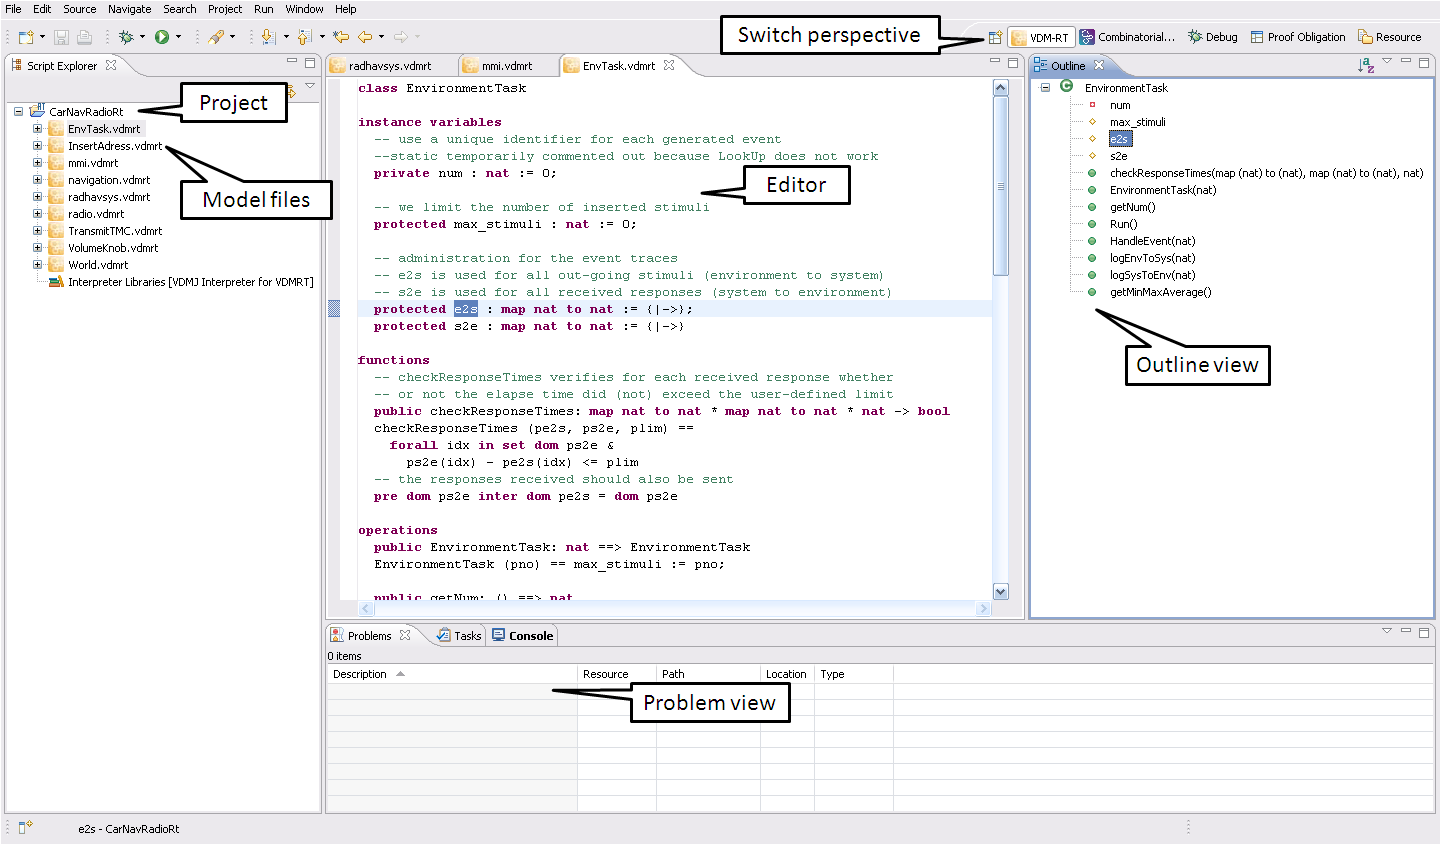
\includegraphics[width=4.5in]{figures/OverturePerspectiveRT}
  \caption[labelInTOC]{The Overture Perspective}
  \label{fig:userguire:OverturePerspective}
\end{center}
\end{figure}

The \emph{Outline view}, to the right of the editor (see
Figure~\ref{fig:userguide:OutlineView}), displays an outline of the
file selected in the editor. It shows all declared classes, their
instance variables, values, types, functions, operations and traces.
Figure~\ref{fig:userguire:OverturePerspective} shows the outline view
on the right hand side. Clicking on an operation or function in the
outline will move the cursor in the editor view to its definition. At
the top of the outline view there is a button to~(optionally) display
the items in the outline view in alphabetical order.

\begin{figure}[!h]
\begin{center}
  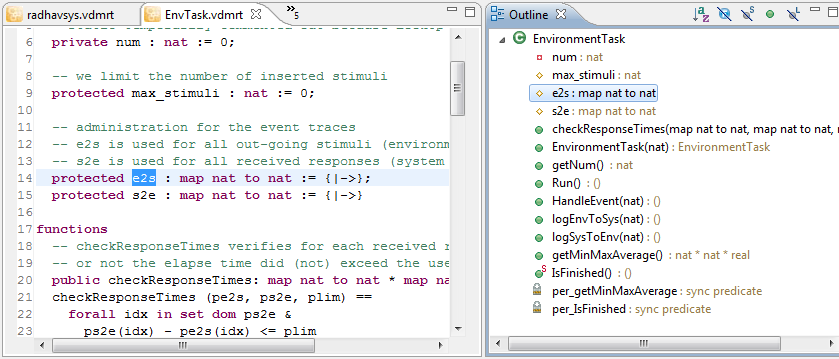
\includegraphics[width=4.5in]{figures/OutlineViewRT}
  \caption[labelInTOC]{The Outline View}
  \label{fig:userguide:OutlineView}
\end{center}
\end{figure}

The \emph{Problems view} presents information about the projects you
are working on, including warnings and error messages. 

Most of the other features of the workbench, such as the menus and
toolbars, are similar to other Eclipse applications, though for
newcomers to Eclipse it is worth noting that there is a special menu
with Overture-specific functionality. One convenient feature is a
toolbar of shortcuts to switch between different perspectives that
appears on the right side of the screen; these vary dynamically
according to context and history.

When making corrections to the model, you can use the Overture IDE
templates. When you hit the key combination \textit{CTRL+space} after
entering the initial characters of the template needed, Overture will
offer possible completions. For example, if you typ ''op'' followed by
\textit{CTRL+space}, Overture will propose the use of an implicit or
explicit operation template.

\begin{figure}
	\begin{center}
	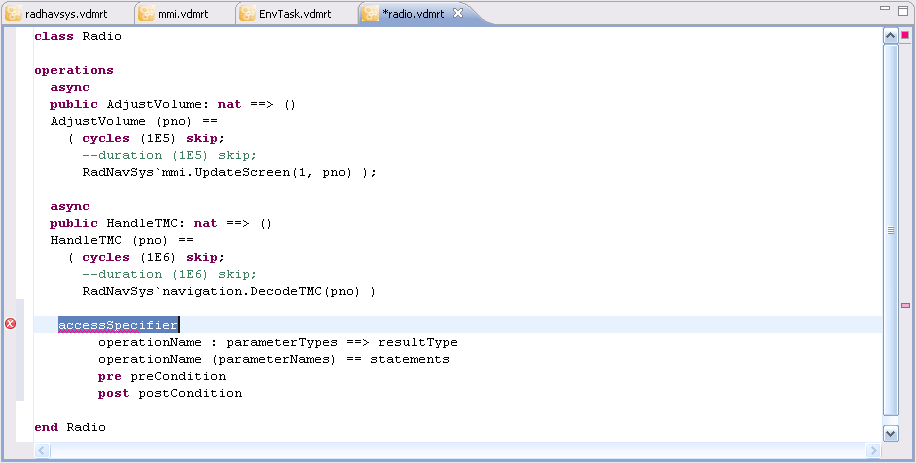
\includegraphics[width=4in]{figures/OperationTemplateRT}
	\caption{Explicit operation template}
	\label{fig:userguide:operationTemplate}
	\end{center}
\end{figure}

The Overture IDE supports many templates for language constructs
including cases statements, classes, quantified expressions, functions
(explicit/implicit), operations (explicit/implicit) and many
more\footnote{It is possible to see and enhance the complete list of
  these by selecting \emph{Window} $\rightarrow$ \emph{Preferences}
  $\rightarrow$ \emph{Overture}.}. Further templates can easily be added in the future. The use of
templates makes it more concenient to write VDM models without
detailed prior knowledge of the language syntax.

When editing a VDM model, the Overture IDE parses the content of the
editor buffer continuously as changes are made. If there are any
syntax errors, these will be reported in the problems view, as well as
being highlighted in the editor. See the bottom of
Figure~\ref{fig:userguire:OverturePerspective}. Each time a
VDM-RT model file is saved the editor type checks the model and reports
any errors or warnings. Note also that the suggestions made about
missing characters in the
error messages may not always be entirely the action you may wish to
take when correcting the source since the tool cannot guess what you
intended to write.

%Most of the imported files in the car navigation project should be
%syntactically correct, but the \texttt{World.vdmrt} file contains one
%deliberate syntax error. The error in this case is a common one: a
%semicolon separating the different definitions has been forgotten.

%\begin{myhardexercise}\label{ex:type-errors}
%Correct all the errors discovered by the type checker and syntax and
%type check your corrected files until no errors appear.
%\textbf{Hint:} Consult the model presented in 
%Appendix~\ref{app:navigation}
%to see how values (note using ``\vdmstyle{=}'' rather than
%``\vdmstyle{:=}''), types and constructors should be defined and how
%access modifiers should be used.
%\end{myhardexercise}


\section{Mapping UML to  VDM}\label{sec:fromUMLtoVDM}\label{sec:syntaxcheck}
\label{sec:typecheck}

In order to map the UML class diagram created in Enterprise Architect
to VDM, a new project must be created in the Overture IDE to receive
it. This is done by right-clicking in the \emph{Script Explorer} view,
and creating a new VDM-RT project and for example naming it
\texttt{CarRadioNavUML}. If the desired language dialect (say a VDM-RT 
project) is not directly available in the right-click menu, please choose
\emph{Project} or 
\emph{Other} and browse to the VDM-RT project. By right-clicking the new 
project root in the \emph{Script Explorer}, \emph{UML Transformation} can 
be chosen, followed by \emph{Import XMI}. Now browse to the XMI/XML file
exported from EA called \texttt{carradnavuml.xmi} and open this.

%The three classes from the Alarm system will be converted to VDM++ format
%(\texttt{.vdmpp}), one file per class.

%When editing a model, it can be useful to navigate to a specific
%operation in the file, instead of reaching for the mouse, this can be
%done using a shortcut (\textit{Ctrl+O})) which opens a small pop-up. This
%pop-up allows the user to navigate to a given location in the model
%simply by filling out the name of an field, operation, function or
%type. The use of intellisense furthermore ensures that the user does
%not have to write out the full name of the desired location. Figure
%\ref{fig:quickOutline} shows the quick outline.

%\begin{figure}
%	\begin{center}
%	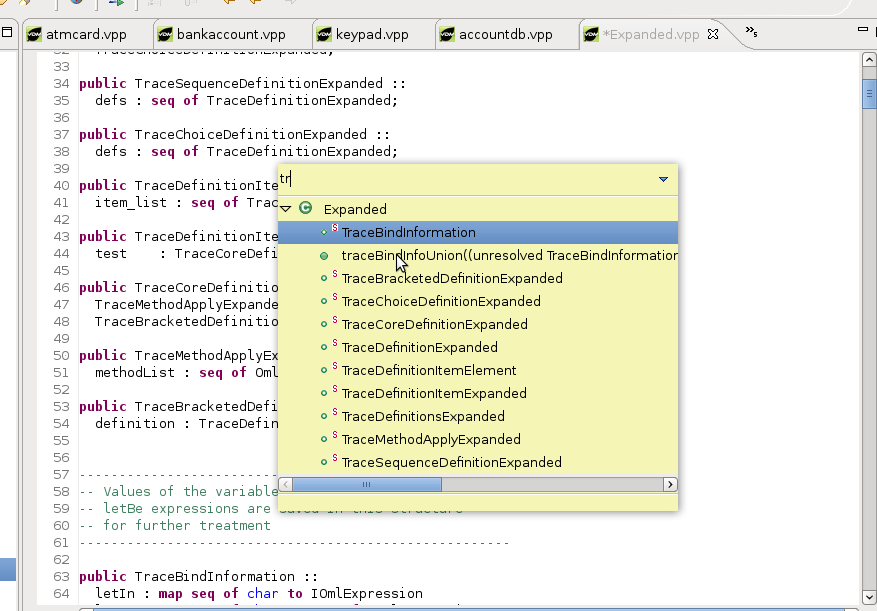
\includegraphics[width=300px]{figures/quickOutline}
%	\caption[Quick Outline]{Quick Outline}
%	\label{fig:quickOutline}
%	\end{center}
%\end{figure}

The transformation from UML to VDM is not entirely automated right now. For
example, any custom types are transformed to VDM++ definitions using
machine-generated identifiers since custom types are not named in
UML. As a result, you have to expect to make minor modifications to
the generated VDM files. 

\subsection{Mapping VDM to UML}

It is possible to automatically transform all the classes from the car
radio navigation project to UML. To do this, simply right
click the project root and choose \emph{UML Transformation} $
\rightarrow $ \emph{Export XMI}. The XMI file can subsequently be
imported in EA, enabling the user to get an overview
of the complete model.

\section{Debugging}\label{sec:debugging}

This section describes how to debug a model by testing it using the
Overture IDE. The model can be exercised by running the operations
\emph{RunScenario1} or \emph{RunScenario2} in the \emph{World} class:

\begin{lstlisting}
class World

types
  
public perfdata = nat * nat * real

instance variables

static public envTasks : map seq of char 
                         to EnvironmentTask := {|->};

operations

addEnvironmentTask: seq of char * EnvironmentTask ==> ()
addEnvironmentTask (pnm, penv) ==
( envTasks := envTasks munion { pnm |-> penv };
  penv.Run() );

public RunScenario1 : () ==> map seq of char 
                             to perfdata
RunScenario1 () ==
( addEnvironmentTask("VolumeKnob", 
                     new VolumeKnob(10));
  addEnvironmentTask("TransmitTMC", 
                     new TransmitTMC(10));
  return { name |-> envTasks(name).getMinMaxAverage() 
         | name in set dom envTasks } );
...
end World
\end{lstlisting}

\subsection{The Debug configuration}

Before you start to debug a model in Overture, you need to set up a
\emph{debug configuration}. Right click the project and choose
\emph{Debug As} $ \rightarrow $ \emph{Debug configuration}\footnote{Note that the
  \emph{Run As} functionality existing Eclipse users are used to is
  not supported in the current version of Overture. In the current
  version of Overture debugging of VDM-RT models in general does not
  work very well because of the scheduling done internally in the
  interpreter. This is currently being redesigned and it is expected
  that in the next stable release this will be fully operational.}. The dialog
requires the project name, the class, the operation/function used as
the entry point of the test and the source file containing the entry
point definition.  As an example,
Figure~\ref{fig:userguide:debugConfiguration} shows the debug
configuration for the car navigation model. The class and
operation/function name can be chosen from a Browse dialog. If the
operation or function has arguments, these must be typed in manually
between the brackets of the entry point function/operation.

\begin{figure}[htp]
\begin{center}
  \includegraphics[width=4in]{figures/DebugConfigurationRT}
  \caption{The debug configuration dialog}
  \label{fig:userguide:debugConfiguration}
\end{center}
\end{figure}

Once the configuration is ready, the model can be debugged. The
Overture IDE will change to the \emph{Debug perspective} which
contains the views needed for debugging in VDM. Breakpoints can easily
be set by double clicking in the left margin of the editor view. When
the debugger reaches a breakpoint, evaluation suspends and the user
can inspect the values of different variables and step through the VDM
model line by line.
 
The Debug perspective is illustrated on figure~\ref{fig:userguide:DebuggingVDM}
\begin{figure}[htp]
\begin{center}
  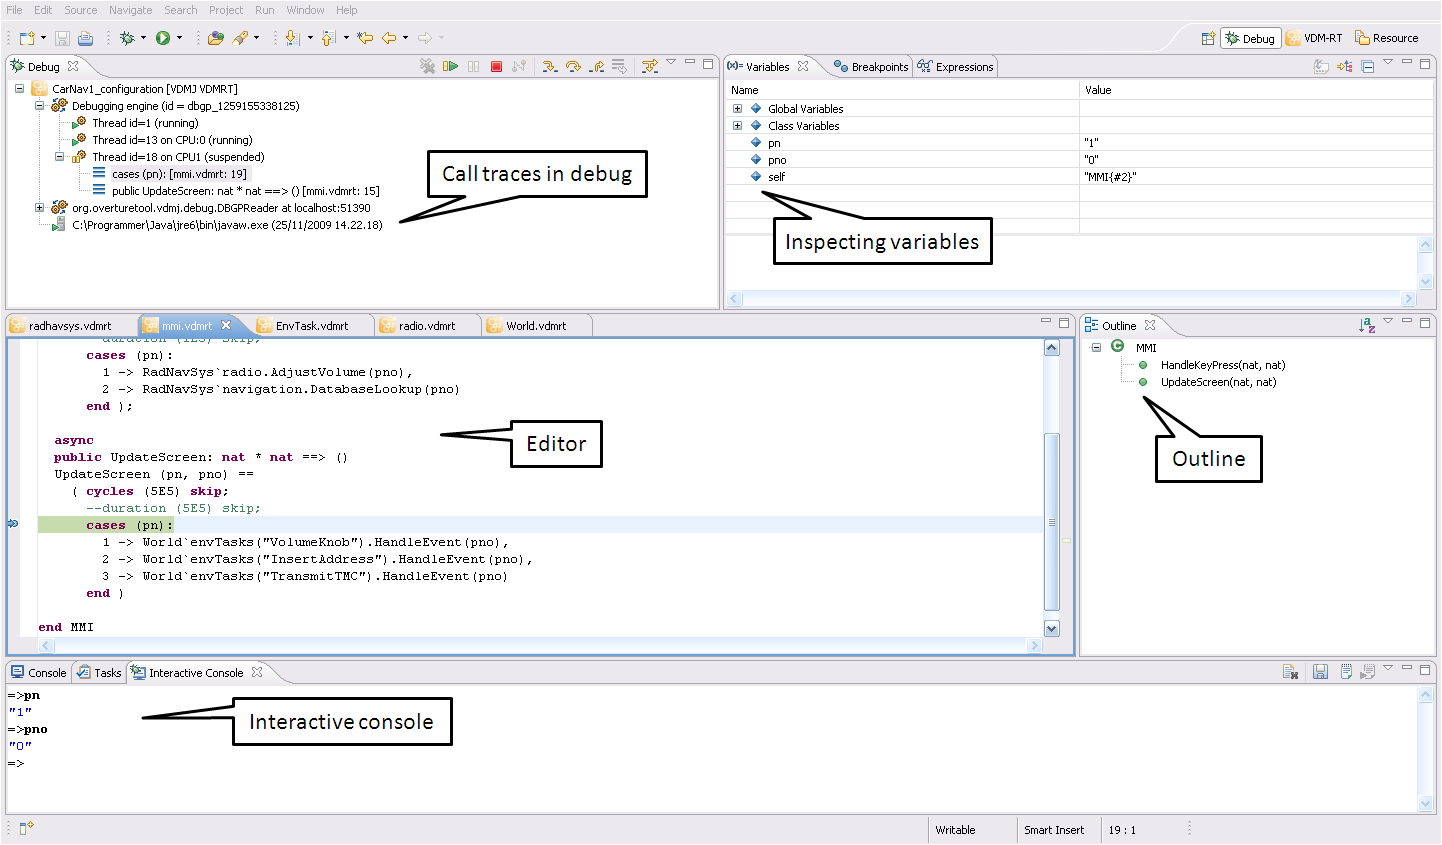
\includegraphics[width=4.5in]{figures/DebuggingVDMRT}
  \caption[Debugging perspective]{Debugging perspective}
  \label{fig:userguide:DebuggingVDM}
\end{center}
\end{figure}
The \emph{Debug view} in the upper left corner of the Debug
perspective shows all running models and their call stacks. It also
shows whether a given model is stopped, suspended or running. All
threads are also shown, along with their running status. It is
possible to switch between threads from the Debug view.

\begin{table}
\begin{center}
\caption{Overture debugging buttons\label{tab:debugButtons}}
\begin{tabular}{|l|l|}\hline \hline
\textbf{Button} & \textbf{Explanation} \\ \hline

\includegraphics[width=0.03\textwidth]{figures/resume} & Resume debugging \\

\includegraphics[width=0.03\textwidth]{figures/suspend} & Suspend debugging\\

\includegraphics[width=0.03\textwidth]{figures/terminate} & Terminate debugging\\

\includegraphics[width=0.03\textwidth]{figures/stepinto} & Step into\\

\includegraphics[width=0.03\textwidth]{figures/stepover} & Step over \\

\includegraphics[width=0.03\textwidth]{figures/stepreturn} & Step return\\

\includegraphics[width=0.03\textwidth]{figures/stepbystep} & Use step filters\\
\hline \hline
\end{tabular}
\end{center}
\end{table}

At the top of the view are standard Eclipse buttons (see
Table~\ref{tab:debugButtons}) for controlling debugging, allowing you
to stop, step into, step over and resume.

The \emph{Variables view} in the upper right corner of the Debug
perspective shows all the variables in a given context, when a
breakpoint is reached. The variables and their displayed values are
automatically updated when stepping through a model.

\begin{figure}[htp]
\begin{center}
  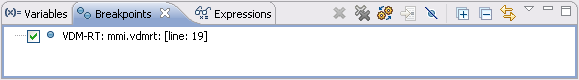
\includegraphics[width=4in]{figures/BreakpointViewRT}
  \caption{Breakpoint View}
  \label{fig:userguide:BreakpointView}
\end{center}
\end{figure}

The \emph{Breakpoints view} gives an overview of all breakpoints
set~(see Figure~\ref{fig:userguide:BreakpointView}). From this view
the user can easily navigate to the location of a given breakpoint,
disable or delete them, or set their properties.
 
%Conditional breakpoints are supported. These are a powerful tool for
%the developer since they allow a condition to be specified which has
%to be true in order for the debugger to stop at the given
%breakpoint. The condition can either be a boolean expression using
%variables in scope at the breakpoint, or it can be a hit count after
%which the breakpoint should become active.

%\begin{figure}[htp]
%\begin{center}
%  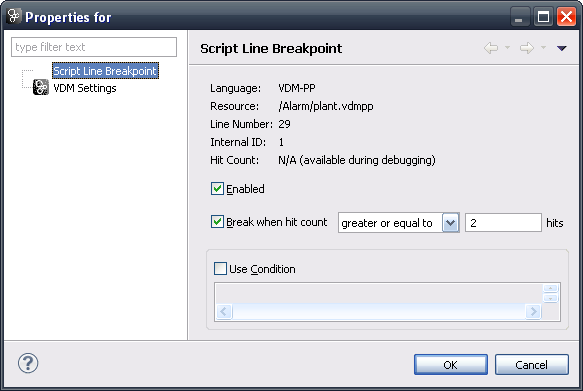
\includegraphics[width=4in]{figures/Breakpointconditional}
%  \caption{Conditional breakpoint options}
%  \label{fig:userguide:BreakpointConditional}
%\end{center}
%\end{figure}

%You can make a simple breakpoint conditional by right clicking on the
%breakpoint mark in the left margin of the editor and selecting the option
%\emph{Breakpoint properties}. This opens a dialog shown in
%figure~\ref{fig:userguide:BreakpointConditional}.

The \emph{Expressions view} allows the user to enter \emph{watch}
expressions whose values are automatically displayed and updated when
stepping. Watch expressions can be added manually or created by
selecting \emph{create watch expression} from the Variables view. It
is possible to edit existing expressions.  Like the Breakpoints view,
this view is hidden in the upper right hand corner in
Figure~\ref{fig:userguide:DebuggingVDM}.

While the Overture Expressions view allows you to easily inspect
values, the functionality is somewhat limited. For more thorough
inspections in Overture, the \emph{Interactive Console view} is
provided. Here commands can be executed in a given context, i.e.\ when
the debugger is at a breakpoint. The Interactive Console keeps a
command history, so that previously executed commands can be run again
easily. The interactive console can be seen at the bottom of
Figure~\ref{fig:userguide:DebuggingVDM}.

\section{Test coverage}\label{sec:testcov}

It is often useful to know how much of a model has been exercised by a
set of tests\footnote{Note that this feature is not yet supported for
  models using unicode characters such a Japanese identifiers.}. 
This gives some insight into the thoroughness of a test
suite and may also help to identify parts of the model that have not
been assessed, allowing new tests to be devised to cover these. When
any evaluation is performed on a VDM-RT model, the interpreter records
the lines of the VDM-RT model that are executed. This permits the line
coverage to be examined after a test to identify the parts of the
VDM++ model that have not yet been exercised -- coverage is
cumulative, so a set of tests can be executed and their total coverage
examined at the end.

In our simple example, the different tests in the exercise above does
cause the majority of the VDM-RT model to be executed, but for
demonstration purposes let us start by cleaning the model (right click
on the project and select \texttt{Clean}). Let us evaluate the
\texttt{RunScenario1} and \texttt{RunScenario2} operations where the
\texttt{Generate test coverage} option is selected. 
Remember that whenever test coverage
information is desired the \texttt{Generate Latex Coverage} option
must be selected as shown in Figure~\ref{fig:debugConfiguration}. 
 Once the debugger
has completed and the result is written out in the \texttt{console} it
is possible to right click on the \texttt{CarRadioNavi} project and
select the \emph{Latex} $ \rightarrow $ \emph{Latex coverage} the
coverage information that have been gathered in any expressions that
have been debugged since the last change to a file have been saved or
the project have been cleaned will be turned into a pdf file. The
\texttt{CarRadioNavi.pdf} file is placed in the
\texttt{generated/latex} directory. Note that whenever the model is
adjusted or it is cleaned so it gets type checked again all the files
in the \texttt{generated} directory is deleted.

The coverage information is provided in a way where uncovered
expressions are shown in red in the generated pdf file. In addition
after the content of each VDM-RT source file a table with coverage
overview is provided in tabular form. So for example for the
\texttt{MMI} class this looks like:

\begin{longtable}{|l|r|r|}
\hline
Function or operation & Coverage & Calls \\
\hline
\hline
HandleKeyPress & 90.0\% & 36 \\
\hline
UpdateScreen & 87.0\% & 65 \\
\hline
\hline
mmi.vdmrt & 88.0\% & 101 \\
\hline
\end{longtable}

\noindent where the \texttt{ExpertIsOnDuty} and \texttt{ExpertToPage} 
operations are fully covered
by just one call (due to the fact that its body is simply one line)
whereas the \texttt{PlantInv} operation is called 2 times.

\section{Realtime Log Viewer}\label{sec:RTLV}

When a VDM-RT model is being executed a textual logfile is created in
a ''\texttt{generated/logs/debugconfig}'' folder with the
\emph{.logrt} extension. This logfile can be viewed in the build-in
RealTime Log Viewer, by double-clicking the file in the project
view. The viewer allows you to explore system execution in different
ways. In Figure~\ref{fig:userguide:ArchitecturalOverview} the
architectural overview of the system is given, describing the
distributed nature of the model.

\begin{figure}[htp]
\begin{center}
  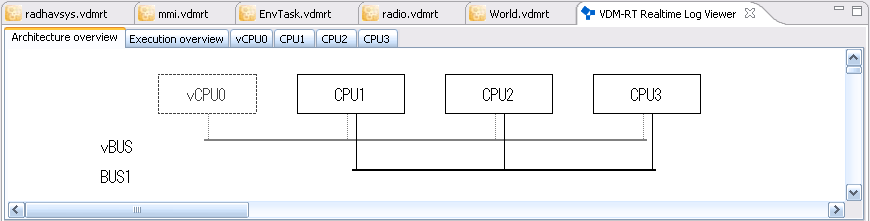
\includegraphics[width=4in]{figures/ArchitectureOverview}
  \caption{Architectural overview}
  \label{fig:userguide:ArchitecturalOverview}
\end{center}
\end{figure}

The RealTime Log Viewer also enables the user to get an overview of
the model execution on a system level -- this can be seen in
Figure~\ref{fig:userguide:ExecutionOverview}. This view shows how the
different CPUs communicate via the BUSes of the system.

\begin{figure}[htp]
\begin{center}
  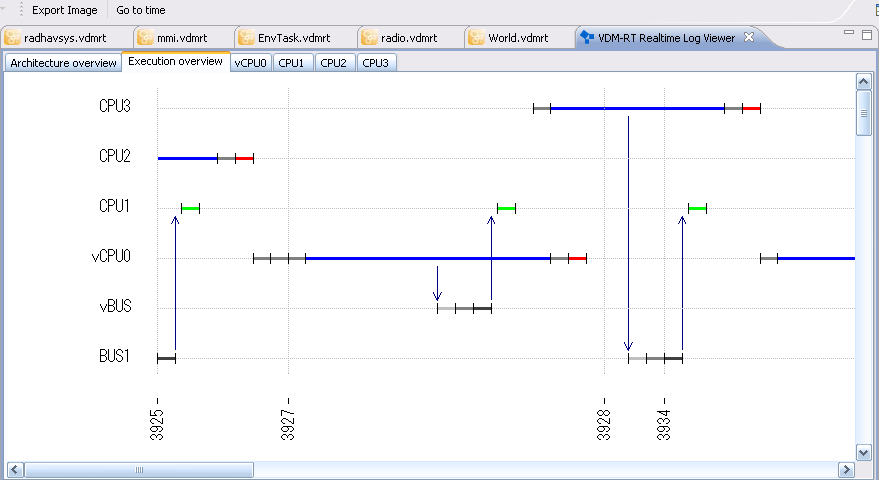
\includegraphics[width=4in]{figures/ExecutionOverview}
  \caption{Execution overview}
  \label{fig:userguide:ExecutionOverview}
\end{center}
\end{figure}

Since the complete execution of the model cannot be shown in a normal
sized window, you have the option of jumping to a certain time
using the \emph{Go to time} button. It is also possible to export all
the generated views to \emph{JPG} format using the \emph{Export Image}
button. All the generated pictures will be placed in the ''log''
folder.

In addition to the execution overview, the RealTime Log Viewer can
also give an overview of all executions on a single CPU. This view
gives a detailed description of all operations and functions invoked
on the CPU as well as the scheduling of concurrent processes. This can
be seen in Figure~\ref{fig:userguide:ExecutionCPU}.

\begin{figure}[htp]
\begin{center}
  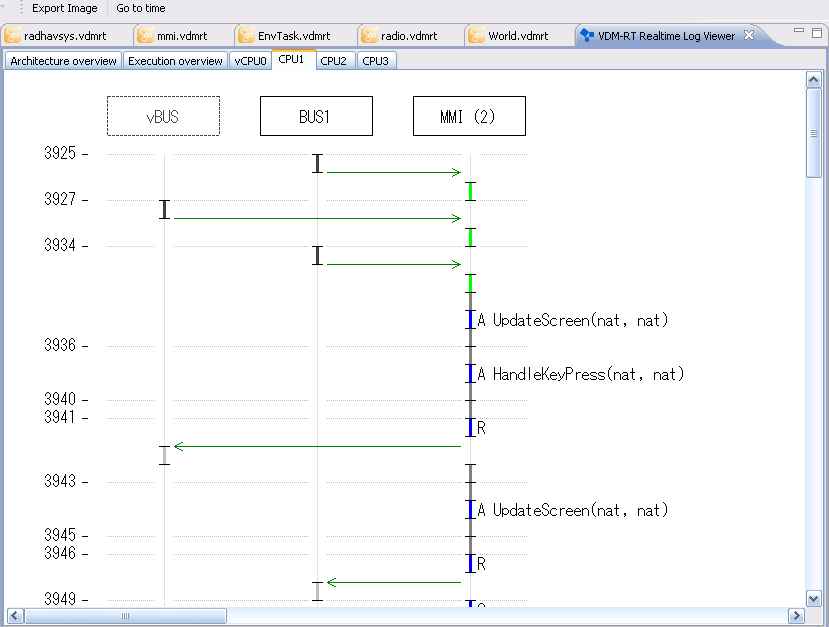
\includegraphics[width=4in]{figures/ExecutionCPU}
  \caption{Execution on single CPU}
  \label{fig:userguide:ExecutionCPU}
\end{center}
\end{figure}

%\section{Combinatorial Testing}\label{sec:CT}

%The previous sections have shown how to manually test and debug models
%that use an executable subset of VDM++. However, Overture also
%contains a feature enabling more automation in the testing process. It
%is possible to write regular expressions, as \emph{traces}, that one
%would like to expand into a large set of individual tests.
%
%In order to illustrate how this can be used, we extend the \texttt{Plant} class
%with two additional operations for adding and removing experts from a given
%schedule. Both operations take a given \texttt{Period} and an \texttt{Expert} and then update the \texttt{schedule} instance variable from the \texttt{Plant}
%class. The \texttt{AddExpertToSchedule} operation can be defined as:
%
%\begin{lstlisting}
%public AddExpertToSchedule: Period * Expert ==> ()
%AddExpertToSchedule(p,ex) ==
%  schedule(p) := if p in set dom schedule
%                 then schedule(p) union {ex}
%                 else {ex};
%\end{lstlisting}

%\noindent and the \texttt{RemoveExpertFromSchedule} operation can
%be expressed as:
%
%\begin{lstlisting}
%public RemoveExpertFromSchedule: Period * Expert ==> ()
%RemoveExpertFromSchedule(p,ex) == 
%  let exs = schedule(p) in
%    schedule := if card exs = 1
%                then {p} <-: schedule
%                else schedule ++ {p |-> exs \ {ex}}
%pre p in set dom schedule;
%\end{lstlisting}

%\noindent Note that \texttt{RemoveExpertFromSchedule} has a deliberate
%error.  It fails to take account of the invariant so this operation
%can leave the \texttt{Plant} in a state where it cannot be guaranteed
%that experts with the right qualifications are available in the
%periods that have been scheduled. \texttt{AddExpertToSchedule} has a
%similar error.  If nobody is scheduled at the period provided as an
%argument, and the expert added for the schedule at this period does
%not have all the necessary qualifications, the invariant will again be
%violated. In fact this means that one would probably have to change
%the signature of this operation such that it instead of taking a
%simple expert would take a collection of experts.  We could use the
%debugger presented above to manually test these two new operations,
%but we can also automate a part of this process.

%In order to do the automation, Overture needs to know about the
%combinations of operation calls that you would like to have carried
%out, so it is necessary to write a kind of regular expression called a
%\emph{trace}. VDM++ has been extended such that traces can be written
%directly as a part of a VDM++ model. A full explanation of this can be
%found at \cite{Larsen&09d}. In our case, inside the \texttt{Test2}
%class one can write:

%\begin{lstlisting}
%traces
%
%AddingAndDeleting: 
%  let myex in set exs
%  in
%    let myex2 in set exs \ {myex}
%    in
%      let p in set ps 
%      in
%       (plant.AddExpertToSchedule(p,myex);
%        plant.AddExpertToSchedule(p,myex2);
%        plant.RemoveExpertFromSchedule(p,myex);
%        plant.RemoveExpertFromSchedule(p,myex2));
%\end{lstlisting}

%\noindent The three nested let-be statements in the trace called
%\texttt{AddingAndDeleting} yield all possible combinations of their variable
%bindings (whereas manual debugging will select an arbitrary few combinations).
%The cardinality of these sets determines the overall number of test cases (each
%being formed as a sequence of four operation calls, as shown). In this case, the
%cardinality of the three sets are respectively 4, 3 and 4. Multiplying these
%gives 48. If you select the Combinatorial Testing perspective you will see the
%\textsf{CT Overview} view. Inside this view one can select the alarm project,
%right click it and choose the \textsf{Run selected} option. Now Overture expands
%and executes all 48 test cases one after each other. The results of these
%executions are illustrated with green check marks and red crosses, meaning that
%the tests passed or failed respectively. See Figure~\ref{fig:stracesalarm}. Note
%that in the Combinatorial Testing perspective, the view in the lower region is
%able to show the individual steps of a selected test case, along with the
%corresponding results from its four operation calls.

%\begin{figure}[htbp]
%\begin{center}
%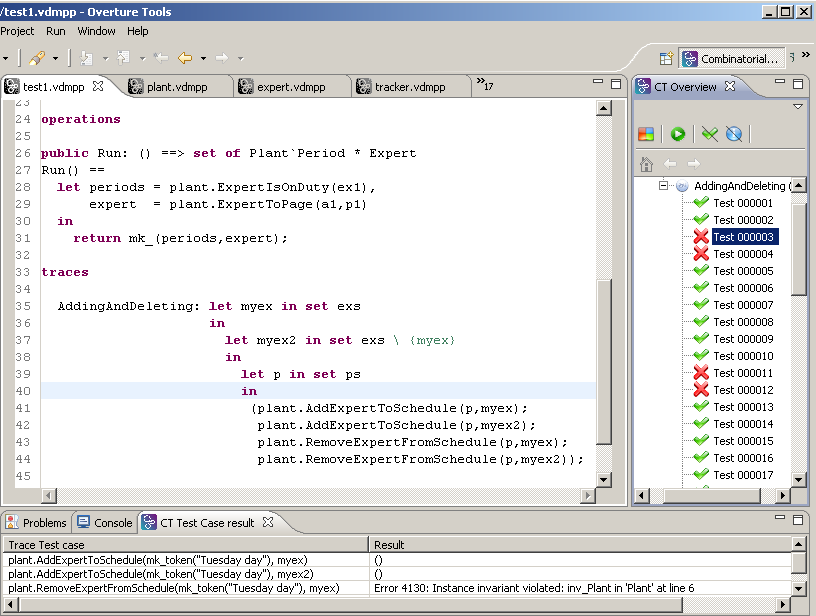
\includegraphics[width=4.5in]{figures/tracesalarm}
%\caption{Using Combinatorial Testing for the Alarm VDM++ model\label{fig:stracesalarm}}
%\end{center}
%\end{figure}
%
%The syntax for traces also enables operation repetition and alternatives to be
%specified, but these were not needed for this simple case. Using the full power
%of traces it is possible to efficiently generate and execute very large test
%suites. Naturally, this is most likely to find inconsistencies when the model
%attempts to define its essential predicates (invariants, pre and post-conditions).

\section{Proof Obligations}\label{sec:PO}

The Overture tool is also able to generate \emph{Proof Obligations}
automatically for VDM-RT models. Proof obligations are boolean
expressions that describe constraints to be met at various points in
the model in order to ensure that the model is internally consistent
(i.e.\ no run-time errors will occur while debugging if these are all
satisfied). Proof obligations are generated to ensure, for example,
that operations will always respect invariants on instance
variables. Each proof obligation generated from a model should
evaluate to \emph{true}.

The proof obligation generator is invoked by right clicking on the
project in the \emph{Explorer view} and then selecting the \emph{Proof
  Obligations} \texttt{->} \emph{Generate Proof Obligations}
entry. This will start up a proof obligation perspective with a
special \emph{PO view}. For the alarm example this view takes the form
shown in Figure~\ref{fig:POview}.

\begin{figure}[htbp]
\begin{center}
\includegraphics[width=4.5in]{figures/POviewRT}
\caption{The Proof Obligation view for the Car Navigation VDM-RT model\label{fig:POview}}
\end{center}
\end{figure}

One of the first proof obligations listed for this example is related
to the \texttt{RunScenario1} operation, which is defined as:

\begin{lstlisting}
public RunScenario1 : () ==> map seq of char to perfdata
RunScenario1 () ==
 (addEnvironmentTask("VolumeKnob", new VolumeKnob(10));
  addEnvironmentTask("TransmitTMC", new TransmitTMC(10));
  return { name |-> envTasks(name).getMinMaxAverage() 
         | name in set dom envTasks } );
\end{lstlisting}

The proof obligation records the constraint that the mapping
application \texttt{envTasks(name)} is indeed defined (i.e.\ that the
\texttt{name} is in the domain of the mapping \texttt{envTasks}). This is described as a proof
obligation in the following form:

\begin{lstlisting}
forall name in set (dom envTasks) &
  name in set dom envTasks
\end{lstlisting}
Proof obligations represent checks that should be made on a model in
order to gain confidence in its consistency. At present, proof
obligations have to be checked by manual inspection of the model
code. Tools are being developed for Overture to check as many as
possible of the proof obligations automatically, but there are always
likely to be some that have to be checked manually. 


\section{A Command-Line Interface}\label{sec:cmdline}

So far only the graphical user interface of the Overture IDE has been
presented but the engine underlying Overture, called VDMJ, also
provides a simple command line interface.  This is useful for the
automatic batch execution of tests, though the command line also
provides a full set of interactive execution and debugging commands
which can be useful when examining batch tests. The command line also
provides access to tool facilities that have not yet been included in
the Overture IDE.

VDMJ is written in Java, and so to run it from the command line, the
VDMJ jar file \footnote{See the Overture documentation at
  \texttt{sourceforge.net/projects/overture} for the location of the
  jar file.}  should be executed with a Java JRE (version 5 or later):

\lstset{style=tool,language=}
\begin{lstlisting}
java -jar vdmj-2.0.0.jar
\end{lstlisting}

\noindent If the jar file is executed with no further options like this, it will
print a list of available options and exit. The most important option is the VDM
dialect that the tool should use. In the case of our alarm example, we want to
use VDM-RT for which the option is \verb|-vdmrt|. After this, we can simply
specify the names of the VDM-RT model files to load, or the name of a directory
in which all the files reside:

\begin{lstlisting}
java -jar vdmj-2.0.0.jar -vdmrt CarNaviRadio
\end{lstlisting}

\noindent That will perform a syntax and type check of all the VDM-RT model
files in the directory \verb|CarNaviRadio|, producing any errors and warning
messages on the console, before terminating:

\begin{lstlisting}
Parsed 9 classes in 0.61 secs. No syntax errors
Type checked 11 classes in 0.093 secs. No type errors
Initialized 11 classes in 0.079 secs. 
\end{lstlisting}

\noindent In the case of our example, there are no syntax or type checking
errors. Warnings can be suppressed using the \verb|-w| option.

If a VDM-RT model has no type checking errors, it can either be given an
expression to evaluate as an option on the command line, or the user can enter
an interactive mode to evaluate expressions and debug their execution.

To evaluate an expression from the command line, the \verb|-e| option is used,
followed by a VDM expression to evaluate. You may also find the \verb|-q|
option useful, as this suppresses the informational messages about the parsing
and type checking:

\begin{lstlisting}
java -jar vdmj-2.0.0.jar -vdmrt -w -q -e 
    "new World().RunScenario1()" CarNaviRadio
\end{lstlisting}

\noindent This produces a single line of output for the evaluation, since the
parsing and checking messages are suppressed, as are the warnings:

\begin{lstlisting}
{"TransmitTMC" |-> mk_(3904, 12574, 6836.25),
 "VolumeKnob" |-> mk_(3935, 16268, 8106.416666666667)}
\end{lstlisting}

Clearly a batch of test evaluations could be performed automatically by running
a series of similar commands and saving the output results for comparison
against expected results.

To run the command line interpreter interactively, the \verb|-i| command line
option must be given. Instead of terminating after the type check, this will
cause VDMJ to enter its interactive mode, and give the interactive \verb|>|
prompt:

\begin{lstlisting}
Parsed 9 classes in 0.61 secs. No syntax errors
Type checked 11 classes in 0.093 secs. No type errors
Initialized 11 classes in 0.079 secs. 
Interpreter started
>
\end{lstlisting}

\noindent From this prompt, various interactive commands can be given to
evaluate expressions, debug their evaluation, or examine the VDM-RT model environment.
The \verb|help| command lists the commands available. The \verb|quit| command
leaves the interpreter.

For example, the following session illustrates the creation of a test object,
followed by an evaluation of its \verb|RunScenario2| operation, and a debug
session with a breakpoint at the start of the same operation:

\begin{lstlisting}
> create world := new World()
> p world.RunScenario2()
= {"InsertAddress" |-> mk_(3993, 16132, 7759.2727272727),
   "TransmitTMC" |-> mk_(3871, 12128, 6980.714285714285)}
Executed in 0.312 secs.

> break World`addEnvironmentTask
Created break [1] in 'World' (CarNaviRadio\World.vdmrt) 
at line 12:5
12:      ( envTasks := envTasks munion { pnm |-> penv };

> p world.RunScenario2()
Stopped break [1] in 'World' (CarNaviRadio\World.vdmrt) 
at line 12:5
12:      ( envTasks := envTasks munion { pnm |-> penv };
[thread 1]> print penv
penv = InsertAddress{#77, max_stimuli:=10, e2s:={|->},
 s2e:={|->},EnvironmentTask{#76, max_stimuli:=10, num:=0,
 e2s:={|->},s2e:={|->}}}
[thread 1]> continue
Runtime: Error 4021: Duplicate map keys have different 
values:
    "InsertAddress" in 'World' (CarNaviRadio\World.vdmrt) 
at line 12:28
Stopped in 'World' (CarNaviRadio\World.vdmrt) 
at line 12:28
12:      ( envTasks := envTasks munion { pnm |-> penv };
[thread 1]> continue
> \end{lstlisting}

\noindent Notice that the \verb|print| command is available at the breakpoint
to examine the runtime state of the system. In the example, we show the value
of the \verb|penv| variable. Continuing from this point, the VDM-RT model
raises a runtime error because the previous execution's results are still in
the (static) \verb|envtasks| map. The VDM-RT model can be re-initialized
between runs with the \verb|init| command to avoid this.

The \verb|help| command is context sensitive, and will list the extra debugging
commands available at a breakpoint, such as \verb|continue|, \verb|step|,
\verb|stack|, \verb|list| and so on. The full set of commands is described in the
VDMJ User Guide\footnote{Supplied with the Overture documentation.}.

\lstset{style=mystyle}

\lstset{style=mystyle,language=VDM++}

\section{Summary}\label{sec:toolintrosummary}

This chapter has introduced the following major features of tool
support for VDM-RT:
\begin{itemize}
%\item using Enterprise Architect with class diagrams\sindex{Enterprise
%  Architect@\tool{Enterprise Architect$^{\mbox{\small\textbf{{\textregistered}}}}$}};
%\item mapping back and forth between Enterprise Architect and Overture;
%\item configuration of selected VDM++ files;
\item syntax checking of VDM-RT models;
\item type checking of VDM-RT models;
%\item the notion of error messages;
\item executing and debugging VDM-RT models;
%\item a command-line interface;
%\item pretty printing VDM++ models with test coverage information;
\item combinatorial testing enabling automation of parts of the
  testing process; 
\item proof obligation generation and
\item a command-line interface enabling access to test coverage.
\end{itemize}


%\backmatter
\appendix

\bibliographystyle{newalpha}

\bibliography{book}

\chapter{A Car Navigation System Example}\label{app:navigation}

This section presents the requirements for a in-car radio navigation system which supports the Traffic Message Channel (TMC). It forms a running example that serves to illustrate the process described earlier and to introduce elements of the VDM++ modelling language with the Real-time extension VICE. Although the modelling process is described here as though it were a single-pass activity, a real development would usually be iterative. 

%%\section{An informal description}

%%Chapter~\ref{cha:toolbox} provides an interactive and hands-on tour of
%%the tools available for supporting the development of the model.

%%The system is composed of three main clusters of functionality; 
%%\begin{itemize}
%%\item The man-machine interface (MMI) takes care of user interaction such as handling key press input and graphical display output. 
%%\item The navigation is responsible for destination entry, route planning and turn-by-turn guidance. 
%%\item The radio is responsible for basic tuner and volume control as well as handling traffic information from the TMC.
%%\end{itemize}

%%The system must be able to support the following three use cases:

%%\begin{description}
%%\item[Change Volume:] The user turns the rotary button and expects near instant audible feedback form the system. Furthermore, the visual feedback
%%(the volume setting on the screen) should be timely and synchronized with the
%%audible feedback.
%%\item[Address Look-up:] Destination entry is supported by a smart �typewriter� style interface. By turning a knob the user can move from letter to letter; by pressing it the user will select the currently highlighted letter. The map database is searched for each letter that is selected and only those letters in the on-screen alphabet are enabled that are potential next letters in the list.
%%\item[TMC Message Handling:] Digital traffic information is important for in-car radio navigation systems. It enables features such as automatic re-planning of the planned route in case a traffic jam occurs ahead. It is also increasingly important to enhance road safety by warning the driver, for example when a ghost driver is spotted just ahead on the planned route. TMC is such a digital traffic information service.
%%\end{description}

\section{System Overview of the Car Navigation example}

In Figure~\ref{fig:navigationoverview} an overview of the in-car
navigation system is shown. Similarily Figure~\ref{fig:worldenv}
provides an overview of the \texttt{World} class and the environment
classes. 

\begin{figure}[!htb]
\begin{center}
  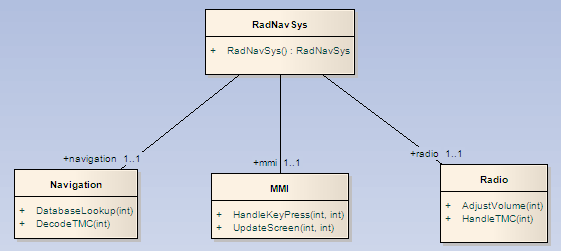
\includegraphics[width=5in]{figures/carnavsys}
  \caption[labelInTOC]{Car Navigation System Overview}
  \label{fig:navigationoverviewapp}
\end{center}
\end{figure}

\begin{figure}[!htb]
\begin{center}
  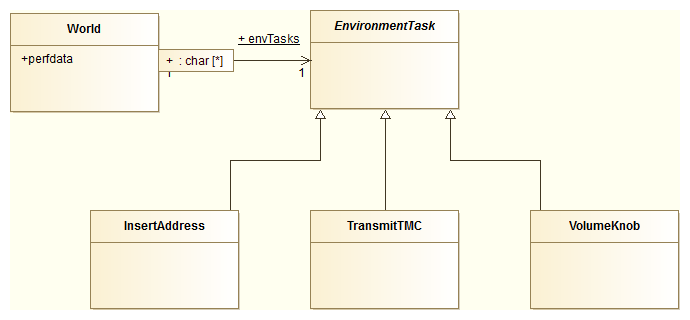
\includegraphics[width=5in]{figures/worldenv}
  \caption[labelInTOC]{Overview of the Wolrd and Environment Classes}
  \label{fig:worldenv}
\end{center}
\end{figure}

\section{The Radio Navigation System Class}

The \texttt{RadNavSys} class is the system class that all VDMRT models must include. 

\begin{lstlisting}
system RadNavSys

instance variables
  -- create an MMI class instance
  static public mmi : MMI := new MMI();
  -- define the first CPU with fixed priority 
  -- scheduling and 22E6 MIPS
  CPU1 : CPU := new CPU (<FP>, 22E6);

  -- create an Radio class instance
  static public radio : Radio := new Radio();
  -- define the second CPU with fixed priority 
  -- scheduling and 11E6 MIPS
  CPU2 : CPU := new CPU (<FP>, 11E6);

  -- create an Navigation class instance
  static public navigation : Navigation := new Navigation();
  -- define the third CPU with fixed priority 
  -- scheduling and 113 MIPS
  CPU3 : CPU := new CPU (<FP>, 113E6); 

  -- create a communication bus that links the three 
  -- CPU's together
  BUS1 : BUS := new BUS (<CSMACD>, 72E3, {CPU1, CPU2, CPU3})
\end{lstlisting}

\begin{lstlisting}
operations
  public RadNavSys: () ==> RadNavSys
  RadNavSys () ==
    ( -- deploy mmi on CPU1
      CPU1.deploy(mmi,"MMIT");
      CPU1.setPriority(MMI`HandleKeyPress,100);
      CPU1.setPriority(MMI`UpdateScreen,90);
      -- deploy radio on CPU2
      CPU2.deploy(radio,"RadioT");
      CPU2.setPriority(Radio`AdjustVolume,100);
      CPU2.setPriority(Radio`DecodeTMC,90);
      -- deploy navigation on CPU3
      CPU3.deploy(navigation,"NavT");
      CPU3.setPriority(Navigation`DatabaseLookup, 100);
      CPU3.setPriority(Navigation`DecodeTMC, 90)
      -- starting the CPUs and BUS is implicit
    );
end RadNavSys
\end{lstlisting}

\section{The MMI Class}

\begin{lstlisting}
class MMI

operations
  async 
  public HandleKeyPress: nat * nat ==> ()
  HandleKeyPress (pn, pno) ==
    ( cycles (1E5) skip;
      cases (pn):
        1 -> RadNavSys`radio.AdjustVolume(pno),
        2 -> RadNavSys`navigation.DatabaseLookup(pno)
      end );

  async 
  public UpdateScreen: nat * nat ==> ()
  UpdateScreen (pn, pno) ==
    ( cycles (5E5) skip;
      cases (pn):
        1 -> World`envTasks("VolumeKnob").HandleEvent(pno),
        2 -> World`envTasks("InsertAddress").HandleEvent(pno),
        3 -> World`envTasks("TransmitTMC").HandleEvent(pno)
      end )

end MMI
\end{lstlisting}

\section{The Radio Class}

\begin{lstlisting}
class Radio

operations
  async 
  public AdjustVolume: nat ==> ()
  AdjustVolume (pno) ==
    ( cycles (1E5) skip;
      RadNavSys`mmi.UpdateScreen(1, pno) );

  async 
  public HandleTMC: nat ==> ()
  HandleTMC (pno) ==
    ( cycles (1E6) skip;
      RadNavSys`navigation.DecodeTMC(pno) )

end Radio
\end{lstlisting}

\section{The Navigation Class}

\begin{lstlisting}
class Navigation

operations
  async 
  public DatabaseLookup: nat ==> ()
  DatabaseLookup (pno) ==
    ( cycles (5E6) skip;
      RadNavSys`mmi.UpdateScreen(2, pno) );

  async 
  public DecodeTMC: nat ==> ()
  DecodeTMC (pno) ==
    ( cycles (5E5) skip;
      RadNavSys`mmi.UpdateScreen(3, pno) )

end Navigation
\end{lstlisting}

\section{The Environment Task Class}

\begin{lstlisting}
class EnvironmentTask 

instance variables
  -- use a unique identifier for each generated event
  private num : nat := 0;

  -- we limit the number of inserted stimuli
  protected max_stimuli : nat := 0;

  -- administration for the event traces
  -- e2s is used for all out-going stimuli 
  -- (environment to system)
  -- s2e is used for all received responses 
  -- (system to environment)
  protected e2s : map nat to nat := {|->};
  protected s2e : map nat to nat := {|->}

functions
  -- checkResponseTimes verifies for each received response 
  -- whether or not the elapse time did (not) exceed the 
  -- user-defined limit
  public checkResponseTimes: map nat to nat * 
                             map nat to nat * nat -> bool
  checkResponseTimes (pe2s, ps2e, plim) ==
    forall idx in set dom ps2e &
      ps2e(idx) - pe2s(idx) <= plim
  -- the responses received should also be sent
  pre dom ps2e inter dom pe2s = dom ps2e
  
operations
  public EnvironmentTask: nat ==> EnvironmentTask
  EnvironmentTask (pno) == max_stimuli := pno;

  public getNum: () ==> nat
  getNum () ==
  ( dcl res : nat := num; 
    num := num + 1; 
    return res );

  -- Run shall be overloaded to implement the event generation 
  -- loop towards the system. typically, it starts a periodic 
  -- thread
  public Run: () ==> ()
  Run () == is subclass responsibility;

  public HandleEvent: nat ==> ()
  HandleEvent (pev) == is subclass responsibility;
 
  -- logEnvToSys is used to register when an event was inserted 
  -- into the system. Note that the 'time' keyword refers to 
  -- the internal simulation wall clock of Overture
  public logEnvToSys: nat ==> ()
  logEnvToSys (pev) == e2s := e2s munion {pev |-> time};

  -- logSysToEnv is used to register when an event was received 
  -- from the system. Note that the 'time' keyword refers to the 
  -- internal simulation wall clock of Overture
  public logSysToEnv: nat ==> ()
  logSysToEnv (pev) == s2e := s2e munion {pev |-> time};

  -- getMinMaxAverage calculates the minimum, maximum and 
  -- average response times that were observed during execution 
  -- of the model note that getMinMaxAverage is blocked until 
  -- the number of system responses is equal to the number of 
  -- sent stimuli termination is ensured because only a maximum 
  -- number of stimuli is allowed to be inserted in the system, 
  -- so eventually all stimuli can be processed by the system. 
  -- This method only works when each stimulus leads to exactly 
  -- one response, which is the case in this instance.
  public getMinMaxAverage: () ==> nat * nat * real
  getMinMaxAverage () ==
    ( dcl min : [nat] := nil, 
          max : [nat] := nil, 
          diff : nat := 0;
      for all cnt in set dom s2e do
        let dt = s2e(cnt) - e2s(cnt) in
          ( if min = nil then min := dt
            else (if min > dt then min := dt);
            if max = nil then max := dt
            else (if max < dt then max := dt);
            diff := diff + dt );
      return mk_(min, max, diff / card dom s2e) )

public static IsFinished: () ==> ()
IsFinished() == skip;

sync
  -- getNum is mutually exclusive to ensure unique values
  mutex (getNum);
  -- getMinMaxAverage is blocked until all responses have 
  -- been received
  per getMinMaxAverage => card dom s2e >= max_stimuli;

  per IsFinished => #fin(logSysToEnv) > 0;

end EnvironmentTask
\end{lstlisting}

\section{The Insert Address Class}

\begin{lstlisting}
class InsertAddress
  is subclass of EnvironmentTask

operations
  public InsertAddress: nat ==> InsertAddress
  InsertAddress (pno) == max_stimuli := pno;

  public HandleEvent: nat ==> ()
  HandleEvent (pev) == logSysToEnv(pev)
  post checkResponseTimes(e2s,s2e,24000000000);

  public Run: () ==> ()
  Run () == start(self); --,VolumeKnobT);

  createSignal: () ==> ()
  createSignal () ==
    ( dcl num2 : nat := getNum();
      logEnvToSys(num2);
      RadNavSys`mmi.HandleKeyPress(2,num2) )

thread
  periodic (2000,100,1000,0) 
    (createSignal)

end InsertAddress
\end{lstlisting}

\section{The Transmit TMC Class}

\begin{lstlisting}
class TransmitTMC
  is subclass of EnvironmentTask

operations
  public TransmitTMC: nat ==> TransmitTMC
  TransmitTMC (pno) == max_stimuli := pno;

  public HandleEvent: nat ==> ()
  HandleEvent (pev) == logSysToEnv(pev)
  post checkResponseTimes(e2s,s2e,40000000000);

  public Run: () ==> ()
  Run () == start(self); --,TransmitTMCT);

  createSignal: () ==> ()
  createSignal () ==
    ( dcl num2 : nat := getNum();
      logEnvToSys(num2);
      RadNavSys`radio.HandleTMC(num2) )

thread
  periodic (4000,400,3910,0) 
    (createSignal)

end TransmitTMC
\end{lstlisting}

\section{The Volume Knob Class}

\begin{lstlisting}
class VolumeKnob
  is subclass of EnvironmentTask

operations
  public VolumeKnob: nat ==> VolumeKnob
  VolumeKnob (pno) == max_stimuli := pno;

  public HandleEvent: nat ==> ()
  HandleEvent (pev) == logSysToEnv(pev)
  post checkResponseTimes(e2s,s2e,22000000000);

  public Run: () ==> ()
  Run () == start(self); --,VolumeKnobT);

  createSignal: () ==> ()
  createSignal () ==
    ( dcl num2 : nat := getNum();
      logEnvToSys(num2);
      RadNavSys`mmi.HandleKeyPress(1,num2) )

thread
  periodic (1000,50,500,0) 
    (createSignal)

end VolumeKnob
\end{lstlisting}

\section{The World Class}

\begin{lstlisting}
class World

types
  public perfdata = nat * nat * real

instance variables
  static public 
  envTasks : map seq of char to EnvironmentTask := {|->};

operations
  addEnvironmentTask: seq of char * EnvironmentTask ==> ()
  addEnvironmentTask (pnm, penv) ==
    ( envTasks := envTasks munion { pnm |-> penv };
      penv.Run() );

  public RunScenario1 : () ==> map seq of char to perfdata
  RunScenario1 () ==
    ( addEnvironmentTask("VolumeKnob", new VolumeKnob(10));
      addEnvironmentTask("TransmitTMC", new TransmitTMC(10));
      return { name |-> envTasks(name).getMinMaxAverage() 
             | name in set dom envTasks } );

  public RunScenario2 : () ==> map seq of char to perfdata 
  RunScenario2 () ==
    ( addEnvironmentTask("InsertAddress",new InsertAddress(10));
      addEnvironmentTask("TransmitTMC", new TransmitTMC(10));
      return { name |-> envTasks(name).getMinMaxAverage() 
             | name in set dom envTasks } );

end World
\end{lstlisting}

\section{The Test Class}

\begin{lstlisting}
class Test

instance variables

mmi   : MMI        := new MMI();
radio : Radio      := new Radio();
nav   : Navigation := new Navigation();

traces

TT: let x in set {1,2,3}
    in
      ((mmi.HandleKeyPress(x,x) | 
        mmi.UpdateScreen(x,x) | 
        radio.AdjustVolume(x) |
        radio.HandleTMC(x) |
        nav.DatabaseLookup(x) |
        nav.DecodeTMC(x));
       EnvironmentTask`IsFinished())
 
end Test
\end{lstlisting}


\end{document}
